\chapter{Tasks}

In this chapter we will describe the tasks we used to evaluate our model against
others.

\section{Classification}

\subsection{IMDB Sentiment Analysis}

In this task the model is asked to classify a piece of text based on its
sentiment, which is either negative or positive. The texts are anonymized
reviews from the Internet Movie Database\footnote{\url{www.imdb.com}} site
collected together with their human-annotated labels. The resulting dataset is
commonly referred to as IMDB classification or sentiment dataset~\cite{maas11}.

The dataset is split evenly to test and train set, each having 25000 reviews.
The dataset also contains 50000 unlabeled reviews. The label distribution in
both sets is uniform, each of of the two labels is represented by 12500 reviews.

As can be seen from the figure Figure~\ref{fig:imdb_word_token_dist} the reviews
are quite short with only 13.56\% being longer than 512 RoBerta tokens.

\begin{figure}[h]
  \centering
  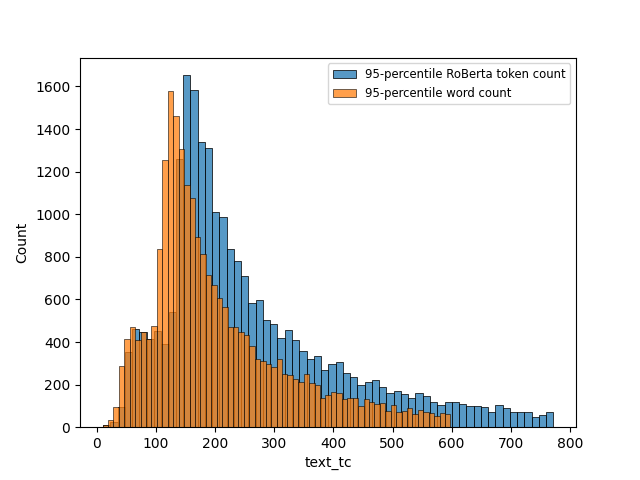
\includegraphics[width=0.9\textwidth]{img/imdb_word_token_distributions.png}
  \caption{Word count and token count distribution of 95-percentiles of
  reviews. The tokens are generated using RoBerta's pretrained tokenizer from
  HuggingFace}\label{fig:imdb_word_token_dist}
\end{figure}


\subsubsection{Doc2Vec}

